\langsection[subsection]{Intersections}{Перекрестки}

\begin{figure}[htbp]
	\centering
	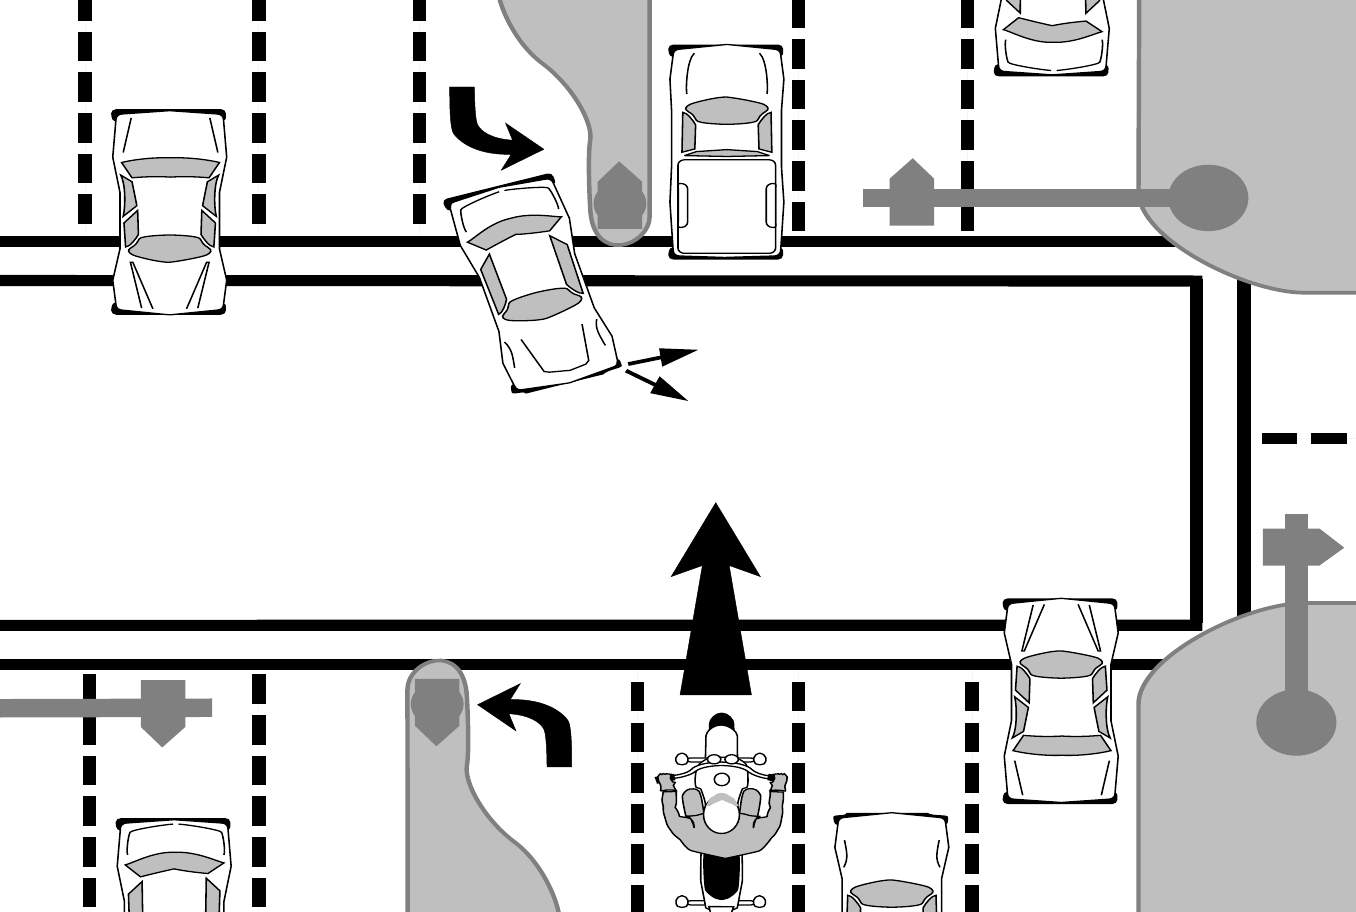
\includegraphics[width=0.9\textwidth, frame]{large_intr}
	\caption{Large intersections}
	\label{fig:large_intr}
\end{figure}



\begin{langblock}{0.425}
	\begin{eng}
	
	The greatest potential for conflict between you and other traffic is at intersections. An intersection can be in the middle of an urban area or at a driveway on a residential street -- anywhere traffic may cross your path of travel. Over one-half of motor- cycle/car crashes are caused by drivers entering a rider's right-of-way. Cars that turn left in front of you, includ- ing cars turning left from the lane to your right, and cars on side streets that pull into your lane, are the biggest dangers. Your use of SEE at intersections is critical.
	
	There are no guarantees that others see you. Never count on eye contact as a sign that a driver will yield. Too often, a driver looks right at a motor- cyclist and still fails to see him. The only eyes that you can count on are your own. If a car can enter your path, assume that it will. Good riders are always looking for trouble -- not to get into it, but to stay out of it.
	
	Increase your chances of being seen at intersections. Ride with your headlight on and in a lane position that provides the best view of oncoming traffic. Provide a space cushion around the motorcycle that permits you to take evasive action.
	
	As you approach the intersection, select a lane position to increase your visibility to the driver.  Cover the clutch lever and both brakes to reduce reaction time.
	
	
	Reduce your speed as you approach an intersection. After entering the intersection, move away from vehicles preparing to turn.  Do not change speed or position radically. The driver might think that you are preparing to turn.
	\end{eng}
	\begin{rus}
		
		Наибольшая вероятность столкновения между вами и другими участниками дорожного движения возникает на перекрестках. Перекресток это и улицы  в центре города и въезд во двор "--- везде, где другие участники дорожного движения пересекают ваш маршрут. Более половины ДТП с участием мотоциклов происходит из-за того, что водители автомобилей не пропустили мотоциклиста. Наибольшую опасность представляют автомобили, поворачивающие налево перед вами, в том числе автомобили, поворачивающие налево с полосы справа от вас, а также автомобили с боковых улиц, выезжающие на вашу полосу движения. Использование парадигмы \textbf{SEE} на перекрестках имеет решающее значение.
		
		Нет никаких гарантий, что вас заметят. Никогда не рассчитывайте на «зрительный контакт» как на признак того, что водитель уступит вам дорогу. Слишком часто водитель смотрит прямо на мотоциклиста, но при этом не «замечает» его. Единственные глаза, на которые вы можете положиться, "--- это ваши собственные. Если автомобиль может выехать перед вами, считайте, что он это сделает. Хорошие мотоциклисты всегда «ожидают неприятности» "--- не для того, чтобы в них попасть, а чтобы их избежать.
		
		Повысьте свои шансы быть замеченным. Езжайте с включенной фарой и занимайте такое положение на полосе, которое обеспечивает наилучший обзор встречного транспорта. Держите вокруг себя интервал\footnote{Формально термин ``a space cushion`` означает «интервал». Если «дистанция» это спереди и сзади, то «интервал» это по сторонам.} с запасом для маневра уклонения.
		
		При приближении к перекрестку выберите положение на полосе движения, которое сделает вас более заметным для других водителей. Держите пальцы на рычагах сцепления и переднего тормоза, а ногу на педали заднего тормоза, чтобы сократить время реакции.
		
		Снизьте скорость при приближении к перекрестку. После въезда на перекресток держитесь подальше от транспортных средств, готовящихся к повороту.  Двигайтесь предсказуемо, не меняйте скорость или положение слишком резко. Водитель может по ошибке подумать, что вы собираетесь повернуть.
\end{rus}
\end{langblock}







\subsubsection{Blind Intersections} 

\begin{figure}[htbp]
	\begin{subfigure}{0.45\textwidth}
		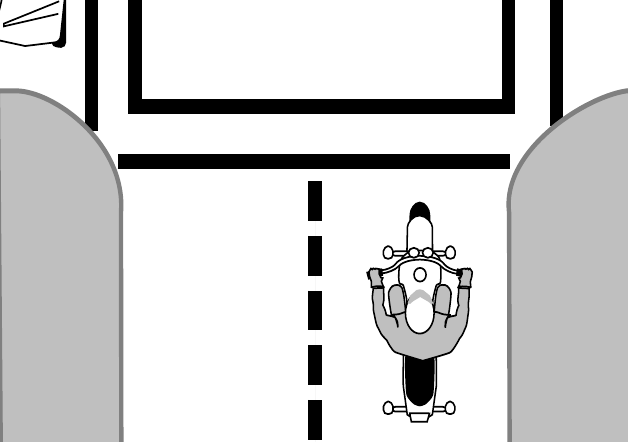
\includegraphics[width=0.95\textwidth, frame]{small_intr}
		\caption{Small intersections}
		\label{fig:small_intr}
	\end{subfigure}
	\hspace*{\fill}
	\begin{subfigure}{0.45\textwidth}
		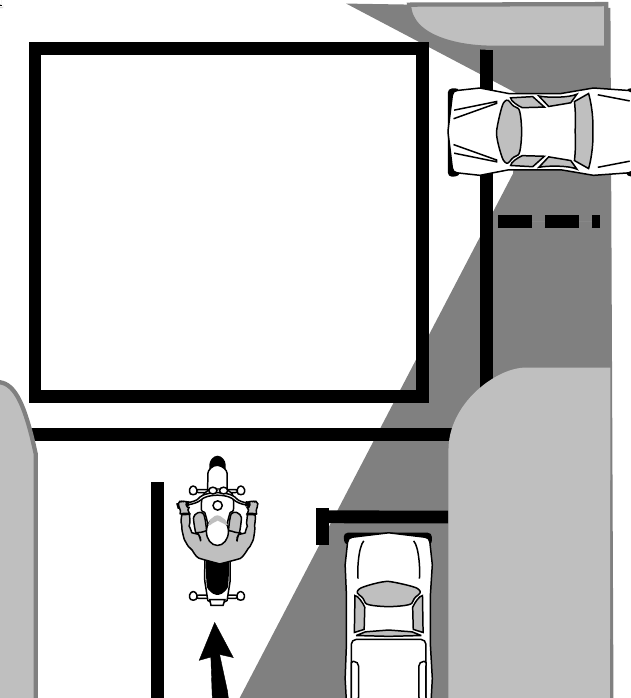
\includegraphics[width=0.95\textwidth, frame]{blind_intr}
		\caption{Blind intersections}
		\label{fig:blind_intr}
	\end{subfigure}
	\caption{Intersections}
	\label{fig:sb_intersections}
\end{figure}


\begin{langblock}{0.425}
	\begin{eng}
	
	If you approach a blind intersection, move to the portion of the lane that will bring you into another driver's field of vision at the earliest possible moment. In this picture \ref{fig:blind_intr} [p. \pageref{fig:blind_intr}], the rider has moved to the left portion of the lane -- away from the parked car -- so the driver on the cross street can see him as soon as possible.
	
	Remember, the key is to see as much as possible and remain visible to others while protecting your space.
	
	If you have a stop sign or stop line, stop there first. Then edge forward and stop again, just short of where the cross-traffic lane meets your lane. From that position, lean your body forward and look around buildings, parked cars, or bushes to see if anything is coming. Just make sure your front wheel stays out of the cross lane of travel while you're looking.
	\end{eng}
	\begin{rus}
		
		Если вы приближаетесь к перекрестку с ограниченной видимостью, переместитесь в ту часть полосы движения, которая позволит вам как можно раньше оказаться в поле зрения другого водителя. На этой фотографии \ref{fig:blind_intr} [с. \pageref{fig:blind_intr}] мотоциклист переместился в левую часть полосы движения "--- подальше от припаркованного автомобиля "--- чтобы другой водитель на перекрестке смог его увидеть как можно раньше.
		
		Помните: главное "--- видеть как можно больше и оставаться заметным для других, одновременно защищая пространство вокруг себя.
		
		Если перед вами есть знак «Стоп» или стоп-линия, сначала остановитесь там. Затем медленно проедьте вперед и снова остановитесь, не доезжая до края перекрестка. Из этого положения наклонитесь вперед и загляните за углы, припаркованные автомобили или кусты, чтобы проверить, не приближается ли что-нибудь. Главное убедитесь, что ваше переднее колесо не находится на перекрестке, пока вы осматриваетесь.
\end{rus}
\end{langblock}





\langsection[subsubsection]{Passing Parked Cars}{Проезд мимо припаркованных автомобилей}

\begin{figure}[htbp]
	\begin{subfigure}{0.4\textwidth}
		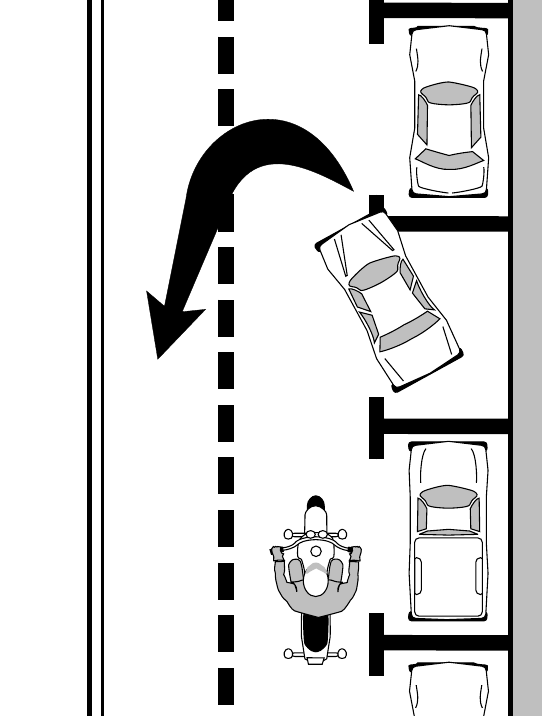
\includegraphics[width=0.95\textwidth, frame]{images/parked_cars.png}
		\caption{Parked cars}
		\label{fig:p_cars}
	\end{subfigure}
	\hspace*{\fill}
	\begin{subfigure}{0.5\textwidth}
		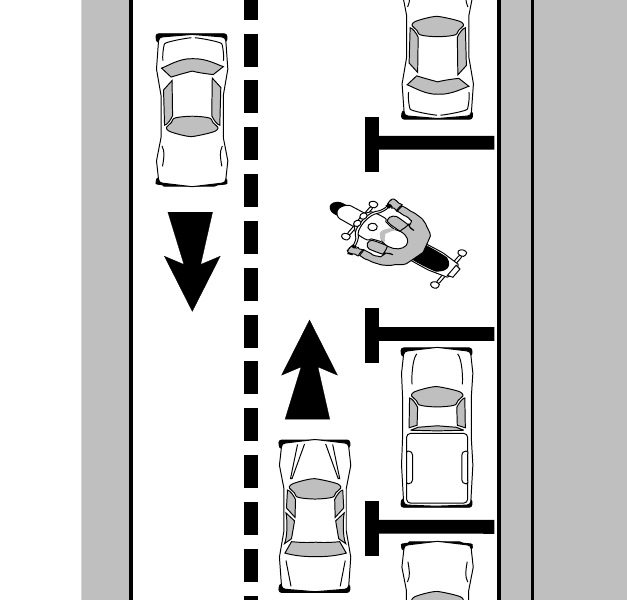
\includegraphics[width=0.95\textwidth, frame]{images/parking_at_curb.png}
		\caption{Parking at curbs}
		\label{fig:p_a_curb}
	\end{subfigure}
	\caption{Parking}
\end{figure}


\begin{langblock}{0.425}
	\begin{eng}
	When passing parked cars, stay toward the left of your lane. You can avoid problems caused by doors opening, drivers getting out of cars, or people stepping from between cars. If oncoming traffic is present, it is usually best to remain in the center-lane position to maximize your space cushion.
	
	A bigger problem can occur if the driver pulls away from the curb without checking for traffic behind.  Even if he does look, he may fail to see you.
	
	In either event, the driver might cut into your path. Slow down or change lanes to make room for someone cutting in.
	
	Cars making a sudden U-turn are the most dangerous. They may cut you off entirely, blocking the whole roadway and leaving you with no place to go. Since you can't tell what a driver will do, slow down and get the driver's attention. Sound your horn and continue with caution.
	\end{eng}
	\begin{rus}
		При езде мимо припаркованных автомобилей держитесь левой части своей полосы, чтобы избежать проблем, связанных с открывающимися дверями, выходящими из машин водителями или людьми, пешеходами выходящими из-за автомобилей. Если есть встречный транспорт, то лучше оставаться в центральной части полосы, чтобы обеспечить максимальный запас для маневра.
		
		Более серьезная проблема, когда водитель начинает трогаться с обочины, не проверив, нет ли кого сзади. И даже если он посмотрит в поисках автомобилей, вас он может просто не заметить.
		
		В любом случае водитель может вклиниться перед вами. Снизьте скорость или перестройтесь в другой ряд и дайте ему проехать.
		
		Наибольшую опасность представляют автомобили, совершающие внезапный разворот. Они могут полностью перекрыть вам путь, заблокировав всю проезжую часть не оставив возможности для маневра. Поскольку вы не можете предсказать действия водителя, снизьте скорость и привлеките его внимание. Посигнальте, продолжайте движение с осторожностью.
\end{rus}
\end{langblock}



\langsection[subsubsection]{Parking at the Roadside}{Правила парковки}


\begin{langblock}{0.425}
	\begin{eng}
	Park at an angle to the curb with your rear wheel touching the curb.
	\end{eng}
	\begin{rus}
		Припаркуйтесь под углом к бордюру так, чтобы заднее колесо касалось бордюра\footnote{Это общее по штату правило. Но например, Филадельфия как обычно имеет много своих особых правил и злых инспекторов желающих выписать вам штраф. То как правильно парковать мотоцикл в вашем городе надо выяснить заранее.}.
\end{rus}
\end{langblock}





































